% Author: Izaak Neutelings (June 2022)
% https://pubs.aip.org/aapt/ajp/article-abstract/91/10/819/2911822/All-objects-and-some-questions?redirectedFrom=fulltext
\documentclass[border=3pt,tikz]{standalone}
\usepackage{amsmath} % for \dfrac
\usepackage{siunitx}
\usepackage[outline]{contour} % glow around text
\contourlength{1.2pt}
\usetikzlibrary{3d} % for canvas
\usetikzlibrary{shadows.blur}
\usetikzlibrary{fadings}
\usetikzlibrary{decorations.text} % for text along path

% STYLE
\tikzset{>=latex}
\tikzstyle{xlab}=[below=-1,scale=0.85]
\tikzstyle{ylab}=[left=-1,scale=0.85]

% COLORS
\colorlet{mydarkblue}{blue!40!black}
\colorlet{mylightblue}{mydarkblue!12} %blue!70!black!20
\colorlet{myred}{red!80!black}
\colorlet{mydarkred}{red!50!black}
\colorlet{mylightred}{mydarkred!12}
\colorlet{mydarkgreen}{green!30!black}
\colorlet{mylightgreen}{mydarkgreen!12}
\colorlet{myorange}{orange!63!black}
\colorlet{mylightorange}{orange!80!black!12}

% CUSTOM HATCHED (denser than default)
\usetikzlibrary{patterns} % for hatched patterns
\def\hatchsize{4pt}
\makeatletter
\pgfdeclarepatternformonly{myhatch}{%
  \pgfqpoint{-1pt}{-1pt}}{\pgfqpoint{\hatchsize}{\hatchsize}}{\pgfqpoint{\hatchsize}{\hatchsize}
}{%
  %\pgfsetcolor{blue!50} %\tikz@pattern@color}
  \pgfsetlinewidth{0.3pt}
  \pgfpathmoveto{\pgfqpoint{0pt}{\hatchsize}}
  \pgfpathlineto{\pgfqpoint{\hatchsize}{0pt}}
  \pgfusepath{stroke}
}
\makeatother

% CUSTOM SHADING
\tikzfading[
  name=fade out,
  inner color=transparent!0,
  outer color=transparent!100
]
\tikzfading[
  name=fade right,
  left color=transparent!0,
  right color=transparent!100
]

% CUSTOM SHADING
% https://tex.stackexchange.com/questions/326542/fill-a-square-with-radial-fading
\usetikzlibrary{shadings}
\makeatletter
\pgfdeclareradialshading[tikz@radial@inner,tikz@radial@outer]%
  {myradial}{\pgfpointorigin}{% \pgfqpoint{-50bp}{-50bp}}{%
    color(0bp)=(pgftransparent!0);%
    color(20bp)=(pgftransparent!90);%
    color(30bp)=(pgftransparent!93);%
    color(40bp)=(pgftransparent!97);%
    color(50bp)=(pgftransparent!100)%
  }
%\pgfdeclareradialshading[tikz@radial@inner,tikz@radial@outer]%
%  {myradial}{\pgfpointorigin}{% \pgfqpoint{-50bp}{-50bp}}{%
%    color(0bp)=(tikz@radial@inner);%
%    color(10bp)=(tikz@radial@outer!50!tikz@radial@inner);%
%    color(25bp)=(tikz@radial@outer!60!tikz@radial@inner);%
%    color(40bp)=(tikz@radial@outer!80!tikz@radial@inner);%
%    color(45bp)=(tikz@radial@outer!90!tikz@radial@inner);%
%    color(50bp)=(tikz@radial@outer)%
%  }
%\pgfdeclareradialshading[tikz@radial@inner,tikz@radial@outer]%
%  {myradial}{\pgfpointorigin}{
%    color(0bp)=(tikz@radial@inner);%
%    color(5bp)=(tikz@radial@outer!10!tikz@radial@inner);%
%    color(20bp)=(tikz@radial@outer!90!tikz@radial@inner);%
%    color(25bp)=(tikz@radial@outer)%
%  }
\makeatother
%\pgfuseshading{sw radial}
\pgfdeclarefading{myradial}{\pgfuseshading{myradial}}%

\begin{document}


% SPACE & TIME SCALES
% Inspiration:
%   "EUREKA!: Physics of Particles, Matter and the Universe", R.J Blin-Stoyle
%   https://aniketvartak.substack.com/p/human-experience-in-a-box?r=b0a55&s=w&utm_campaign=post&utm_medium=web
\def\xmin{-15} % minimum space dimension ~ SM particles (OMG Particle: 1e-27, Planck length: 1.6e−35)
\def\xmax{ 26}    % maximum space dimension ~ observable universe
\def\ymin{-23}    % minimum time dimension ~ SM interactions (Planck time: 5.4e−44)
\def\ymax{18}     % maximum time dimension ~ age of universe ~ 13.8 Bya = 13.8e9*365*24*3600 s
\def\xminhum{-4}  % human experience xmin ~ 1e-4 m ~ 0.1 mm
\def\xmaxhum{7}   % human experience xmax ~ 1e7  m ~ 12,800 km (Earth's diameter)
\def\yminhum{-2}  % human experience ymin ~ 1e-2 s ~ 0.01 s
\def\ymaxhum{10}  % human experience ymax ~ 3e9  s ~ 100 y = 100*365*24*3600 s
\def\tick#1#2{\draw[semithick] (#1) ++ (#2:15pt) --++ (#2-180:30pt)}
\begin{tikzpicture}[
    scale=0.1,x=40,y=40,
    every node/.style={align=center}, % for breaking lines in nodes
  ] % scale such that coordinates coincide with loglog
  
  % HATCHED AREA
  \contourlength{2pt}
  \draw[thick,pattern=myhatch,pattern color=black!80]
    (\xmin,\ymin) rectangle (\xmax,\ymax);
  
  % X AXIS LABELS
  \node[above,rotate=90] at ({\xmin-0.11*(\xmax-\xmin)},{(\ymin+\ymax)/2}) {Time [s]};
  \node[right=4,xlab] at (\xmin,\ymin) {$10^{\xmin}$};
  \node[left=2,xlab] at (\xmax,\ymin) {$10^{\xmax}$};
  
  % Y AXIS LABELS
  \node[below] at ({(\xmin+\xmax)/2},{\ymin-0.05*(\ymax-\ymin)}) {Space [m]};
  \node[above=2,ylab] at (\xmin,\ymin) {$10^{\ymin}$};
  \node[below=2,ylab] at (\xmin,\ymax) {$10^{\ymax}$};
  
  % GUIDE LINES
  \draw (\xminhum,\yminhum) -- (\xminhum,\ymin)
    node[xlab] {$10^{\xminhum}$};
  \draw (\xmaxhum,\yminhum) -- (\xmaxhum,\ymin)
    node[xlab] {$10^{\xmaxhum}$};
  \draw (\xminhum,\yminhum) -- (\xmin,\yminhum)
    node[ylab] {$10^{\yminhum}$};
  \draw (\xminhum,\ymaxhum) -- (\xmin,\ymaxhum)
    node[ylab] {$10^{\ymaxhum}$};
  
  % TICKS
  \tick{\xminhum,\ymin}{90};
  \tick{\xmaxhum,\ymin}{90};
  \tick{\xmin,\yminhum}{0};
  \tick{\xmin,\ymaxhum}{0};
  
  % LABELS
  \draw[thick,fill=white]
    (\xminhum,\yminhum) rectangle (\xmaxhum,\ymaxhum)
    node[midway,align=center,scale=0.88] {
      human\\experience
    };
  \node[below left=1] at (\xmax,\ymax) {
    \contour{white}{observable}\\[-2]
    \contour{white}{universe}
  };
  \node[below] at (-7,7) { % 1d-100y = 8.640e5-3e9 s
    \contour{white}{cells}
  };
  \node[below=4.4] at (2.7,-0.7) { % < 20 km, 1e-3-10s
    \contour{white}{pulsars}
  };
  \node[below] at (\xmaxhum,17) { % 4.543 Bya = 1.433e17 s
    \contour{white}{Earth}
  };
  \node[above right=1] at (\xmin,\ymin) {
    \contour{white}{Standard}\\[-2]
    \contour{white}{Model}\\[-2]
    \contour{white}{interactions}
  };
  
\end{tikzpicture}


% SPACE & TIME SCALES
\begin{tikzpicture}[
    scale=0.1,x=40,y=40,
    every node/.style={align=center}, % for breaking lines in nodes
  ] % scale such that coordinates coincide with loglog
  
  % HATCHED AREA
  \contourlength{2pt}
  \draw[thick,left color=mylightred,right color=mylightblue,
        middle color=white,shading angle=135]
    (\xmin,\ymin) rectangle (\xmax,\ymax);
  
  % X AXIS LABELS
  \node[above,rotate=90] at ({\xmin-0.11*(\xmax-\xmin)},{(\ymin+\ymax)/2}) {Time [s]};
  \node[right=4,xlab] at (\xmin,\ymin) {$10^{\xmin}$};
  \node[left=2,xlab] at (\xmax,\ymin) {$10^{\xmax}$};
  
  % Y AXIS LABELS
  \node[below] at ({(\xmin+\xmax)/2},{\ymin-0.05*(\ymax-\ymin)}) {Space [m]};
  \node[above=2,ylab] at (\xmin,\ymin) {$10^{\ymin}$};
  \node[below=2,ylab] at (\xmin,\ymax) {$10^{\ymax}$};
  
  % GUIDE LINES
  \draw[dashed,mydarkgreen] (\xminhum,\yminhum) -- (\xminhum,\ymin)
    node[xlab] {$10^{\xminhum}$};
  \draw[dashed,mydarkgreen] (\xmaxhum,\yminhum) -- (\xmaxhum,\ymin)
    node[xlab] {$10^{\xmaxhum}$};
  \draw[dashed,mydarkgreen] (\xminhum,\yminhum) -- (\xmin,\yminhum)
    node[ylab] {$10^{\yminhum}$};
  \draw[dashed,mydarkgreen] (\xminhum,\ymaxhum) -- (\xmin,\ymaxhum)
    node[ylab] {$10^{\ymaxhum}$};
  
  % TICKS
  \tick{\xminhum,\ymin}{90};
  \tick{\xmaxhum,\ymin}{90};
  \tick{\xmin,\yminhum}{0};
  \tick{\xmin,\ymaxhum}{0};
  
  % LABELS
  \draw[thick,mydarkgreen,inner color=mylightgreen,outer color=mylightgreen!30]
    (\xminhum,\yminhum) rectangle (\xmaxhum,\ymaxhum)
    node[midway,align=center,scale=0.88] {
      human\\experience
    };
  \node[mydarkblue,below left=-1] at (\xmax,\ymax) {
    observable\\[-2]universe
  };
  \node[below] at (-7,7) {cells}; % 1d-100y = 8.640e5-3e9 s
  \node[below=3] at (2.7,-0.7) {pulsars}; % < 20 km, 1e-3-10s
  \node[below] at (\xmaxhum,17) {Earth}; % 4.543 Bya = 1.433e17 s
  \node[mydarkred,above right=0] at (\xmin,\ymin) {
    \contour{mylightred}{Standard}\\[-2]
    \contour{mylightred}{Model}\\[-2]
    \contour{mylightred}{interactions}
  };
  \fill[mydarkred] (\xmin,\ymin) circle(12pt);
  \fill[mydarkblue] (\xmax,\ymax) circle(12pt);
  
\end{tikzpicture}


% BRONSTEIN CUBE / BRONSHTEIN CUBE
% G (Gravitation), 1/c (Velocity), hbar (Action)
% Inspiration:
%   https://arxiv.org/pdf/1803.02577.pdf
%   http://backreaction.blogspot.com/2011/05/cube-of-physical-theories.html
%   https://www.motionmountain.net/physicscube.html
\begin{tikzpicture}[
    scale=3,y={(0:1cm)},x={(-140:0.65cm)},z={(0,1cm)},
    note/.style={midway,sloped,above,scale=0.5},
    bar/.style={thick,blue!40!black,line cap=round},
    axis/.style={->,bar,black},
    point/.style={mydarkred,canvas is yz plane at x=0},
    point at 1/.style={mydarkred,canvas is yz plane at x=1},
    every node/.style={align=center}, % for breaking lines in nodes
  ]
  \def\R{0.03} % sphere radius
  \def\xmax{1.3}
  
  % FILLS
  \begin{scope}[canvas is xy plane at z=0]
    \fill[mydarkred!20,path fading=fade out,fading transform={shift={(35:1.0)}}]
      (0,-0.2) rectangle (1,1);
    \fill[mydarkred!20,path fading=fade out,fading transform={shift={(-35:1.0)}}]
      (0,-0.2) rectangle (1,1);
    \fill[mydarkgreen!20,path fading=fade out,fading transform={shift={(112:0.8)}}]
      (0,0) rectangle (1.2,1.2);
    \fill[mydarkblue!20,path fading=fade out,fading transform={shift={(-135:1.1)}}]
      (-0.2,0) rectangle (1,1.2);
  \end{scope}
  \begin{scope}[canvas is yz plane at x=0]
    \clip (0,0) rectangle (1,1);
    \draw[left color=mydarkgreen!20,
          right color=white,middle color=white]
      (0,0) rectangle (1.5,1);
    \fill[path fading=fade out,mydarkred!20] (1,0) circle(0.7);
    \fill[path fading=fade out,mydarkblue!20] (1,1) circle(0.7);
      (0,0) rectangle (1,1);
  \end{scope}
  \begin{scope}[canvas is xz plane at y=0]
    \clip (0,0) rectangle (1,1);
    \draw[left color=mydarkblue!20,right color=mydarkgreen!20]
      (0,0) rectangle (1,1);
  \end{scope}
  
  % AXES
  \fill[point] (0,0) circle(\R); % (0,0,0)
  \draw[bar,shorten <=50*\R] (0,0,0) -- (1,0,0);
    %node[note,pos=0.50] {fast motion};
  \draw[bar,shorten <=70*\R] (0,0,0) -- (0,1,0);
    %node[note,pos=0.75] {tiny motion};
  \draw[bar,shorten <=70*\R] (0,0,0) -- (0,0,1);
    %node[note,pos=0.35,below] {bound motion};
  \fill[point] (0,1) circle(\R); % (0,0,1)
  \fill[point] (1,0) circle(\R); % (0,1,0)
  \fill[point at 1] (0,0) circle(\R); % (1,0,0)
  
  % EXTRA BARS
  \draw[axis,shorten <=50*\R] (1,0,0) -- (\xmax,0,0) node[above left=-2] {$1/c$};
  \draw[axis,shorten <=70*\R] (0,1,0) -- (0,\xmax,0) node[above left=0] {$\hbar$};
  \draw[axis,shorten <=70*\R] (0,0,1) -- (0,0,\xmax) node[below left=1] {$G$};
  \draw[bar,shorten <=50*\R] (0,0,1) -- (1,0,1);
  \draw[bar,shorten <=70*\R] (0,0,1) -- (0,1,1);
  \draw[bar,shorten <=70*\R] (1,0,0) -- (1,0,1);
  \draw[bar,shorten <=70*\R] (1,0,0) -- (1,1,0);
  \fill[point at 1] (0,1) circle(\R); % (1,0,1)
  \draw[bar,shorten <=70*\R] (1,0,1) -- (1,1,1);
  \draw[bar,shorten <=70*\R] (0,1,0) -- (0,1,1);
  \draw[bar,shorten <=70*\R] (0,1,0) -- (1,1,0);
  \fill[point] (1,1) circle(\R);
  \draw[bar,shorten <=70*\R] (0,1,1) -- (1,1,1);
  \fill[point at 1] (1,0) circle(\R);
  \draw[bar,shorten <=70*\R] (1,1,0) -- (1,1,1);
  \fill[point at 1] (1,1) circle(\R);
  
  % LABELS
  \node[left=3,below right,scale=0.8] at (0,0,0)
    {Classical\\Mechanics};
  \node[below right,scale=0.8] at (0,0,1)
    {Newtonian\\Gravity};
  \node[left=4,below right,scale=0.8] at (1,0,0)
    {Special\\Relativity};
  \node[below right,scale=0.8] at (1,0,1)
    {General\\Relativity};
  \node[left=2,below right=0,scale=0.8] at (0,1,0)
    {Quantum\\Mechanics};
  \node[below right=-3,scale=0.8] at (1,1,0)
    {Quantum\\Field Theory};
  \node[below=3,right,scale=0.8] at (0,1,1)
    {Non-relativistic\\Quantum Gravity};
  \node[below right=-1,scale=0.8] at (1,1,1)
    %{Theory of\\Everything};
    {Quantum\\Gravity};
  
\end{tikzpicture}


% Plank hyperbola (lP = sqrt(hbar*G/c^3) constant)
% https://arxiv.org/abs/2001.04491
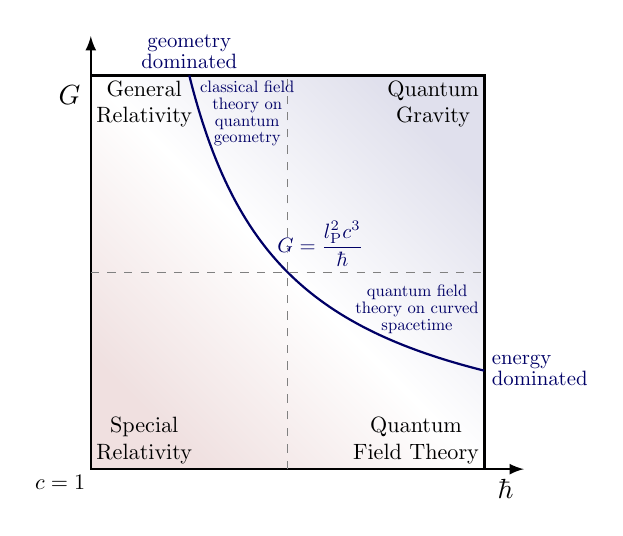
\begin{tikzpicture}[
    scale=5,
    every node/.style={align=center}, % for breaking lines in nodes
  ]
  \def\A{0.25} % hyperbola coefficient
  
  % AXIS
  \draw[thick,left color=mylightred,right color=mylightblue,
        middle color=white,shading angle=135]
    (0,0) rectangle (1,1);
  \draw[<->,thick]
    (1.1,0) node[below left=0] {$\hbar$} -|
    (0,1.1) node[below left=0] at (0,1) {$G$};
  \draw[black!50,dashed] (0.5,0) --+ (0,1);
  \draw[black!50,dashed] (0,0.5) --+ (1,0);
  
  % PLANCK HYPERBOLA (Planck length constant)
  \draw[mydarkblue,thick,domain=\A:1,samples=100]
    plot(\x,\A/\x);
  \node[mydarkblue,above right=-3.5,scale=0.75] at (0.48,\A/0.48) %,rotate=-45
    %{\contour{white}{$l_\mathrm{P}=\sqrt{\dfrac{\hbar G}{c^3}}$}};
    {\contour{white}{$G=\dfrac{l_\mathrm{P}^2c^3}{\hbar}$}};
  
  % REGIME LABELS
  \node[scale=0.8,below left=-1] at (0,0)
    {$c=1$};
  \node[scale=0.8,above right=-1] at (0,0)
    {Special\\Relativity};
  \node[scale=0.8,above left=-1] at (1,0)
    {Quantum\\Field Theory};
  \node[scale=0.8,below right=-1] at (0,1)
    {General\\Relativity};
  \node[scale=0.8,below left=-1] at (1,1)
    {Quantum\\Gravity};
  
  % LABELS
  \node[mydarkblue,scale=0.75,above=0] at (\A,1)
    {geometry\\[-2]dominated};
  \node[mydarkblue,scale=0.75,right=0,align=left] at (1,\A)
    {energy\\[-2]dominated};
  \node[mydarkblue,scale=0.6,right=3,below right=0] at (\A,1)
    {classical field\\[-2] %\contour{mylightblue!70}{classical field}\\[-2]
     theory on\\[-2]
     quantum\\[-2]
     geometry};
  \node[mydarkblue,scale=0.6,above left=0] at (1,\A+0.08)
    {quantum field\\[-2]
     theory on curved\\[-2] spacetime};
  
\end{tikzpicture}


% cGh physics
% Inspiration:
%   https://en.wikipedia.org/wiki/CGh_physics
\usetikzlibrary{shapes} % for cloud
\begin{tikzpicture}[
    xscale=2.8,yscale=2.4,
    myarrow/.style={->,very thick,draw=mydarkgreen},
    myredarrow/.style={myarrow,draw=mydarkred},
    mybluearrow/.style={myarrow,draw=mydarkblue},
    myorangearrow/.style={myarrow,draw=myorange,dashed},
    mynode/.style={thick,draw=mydarkgreen,fill=mylightgreen,rectangle,rounded corners=4,align=center},
    myrednode/.style={mynode,draw=mydarkred,fill=mylightred},
    mybluenode/.style={mynode,draw=mydarkblue,fill=mylightblue},
    myorangenode/.style={mynode,draw=myorange,fill=mylightorange},
    mycap/.style={shorten <=-0.3,line cap=round}
  ]
  
  % ROW 1
  \node[mynode] (CM) at (0,0) {Classical\\Mechanics};
  \node[mynode] (NG) at (1,0) {Newtonian\\Gravity};
  \draw[myarrow] (CM) -- (NG);
  
  % ROW 2
  \node[myrednode] (QM) at (-1,-1) {Quantum\\Mechanics};
  \node[mynode] (EM) at ( 0,-1) {Electro-\\magnetism};
  \node[mybluenode] (SR) at ( 1,-1) {Special\\Relativity};
  \node[mybluenode] (GR) at ( 2,-1) {General\\Relativity};
  \draw[mybluearrow] (SR) -- (EM);
  \draw[mybluearrow] (SR) -- (GR);
  
  % ROW 3
  \node[myrednode] (QF) at (0,-2) {Quantum\\Field\\Theory};
  \node[myorangenode] (CS) at (1,-2) {QFT in\\curved\\spacetime};
  %\node[myrednode,dashed] (QG) at (2,-2) {Quantum\\Gravity};
  \node[myorangenode,cloud,inner sep=0,loosely dashed,
        aspect=1.5,cloud puffs=12,cloud puff arc=170]
    (QG) at (2,-2) {Quantum\\Gravity};
  \draw[myredarrow] (QF) -- (CS);
  \draw[myorangearrow] (CS) -- (QG);
  
  % ARROWS
  \draw[myarrow,mycap] (CM) -- (QM);
  \draw[myarrow,mycap] (CM) -- (SR);
  \draw[myarrow,mycap] (NG) -- (GR);
  \draw[myredarrow,mycap] (QM) -- (QF);
  \draw[myarrow] (EM) -- (QF);
  \draw[mybluearrow,mycap] (SR) -- (QF);
  \draw[myorangearrow] (GR) -- (QG);
  \draw[myorangearrow,shorten <=-0.55] (GR) -- (CS);
  
\end{tikzpicture}


% MR-diagram
% https://arxiv.org/abs/1101.2760
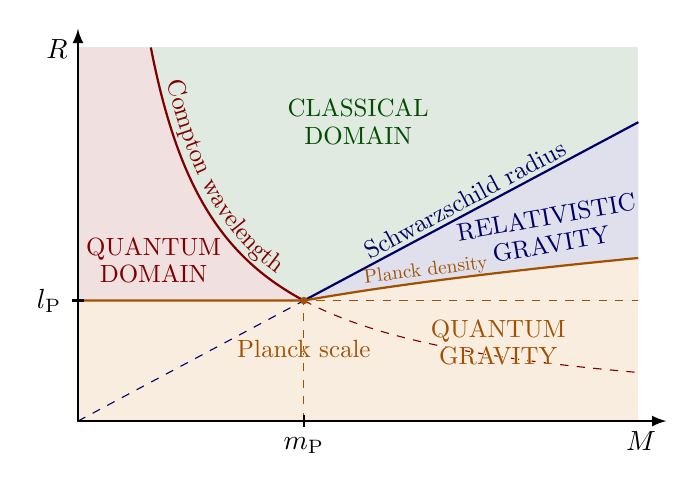
\begin{tikzpicture}[
    scale=4.5,x=45,y=30, % scale such that coordinates coincide with loglog
    every node/.style={align=center}, % for breaking lines in nodes
  ]
  \def\A{0.13} % hyperbola coefficient
  \def\B{0.80} % slope Schwarzschild radius line
  \pgfmathsetmacro\MP{sqrt(\A/\B)} % Planck mass
  \pgfmathsetmacro\LP{sqrt(\A*\B)} % Planck length
  \def\tick#1#2{\draw[thick] (#1) ++ (#2:0.5pt) --++ (#2-180:1pt)}
  \coordinate (P) at (\MP,\LP); % Compton-Schwarschild intersection
  
  % REGION FILLS
  \fill[mylightgreen] (0,0) rectangle (1,1);
  \fill[mylightorange] (0,0) rectangle (1,\LP);
  \fill[mylightblue] (P) -- (1,\B) |- cycle;
  \fill[mylightorange,domain=\MP:1,samples=100]
    (0,0) -- (0,\LP) -- (P) plot(\x,{\LP*(\x/\MP)^(1/3)}) |- cycle;
  \fill[mylightred,domain=\A:\MP,samples=100]
    plot(\x,\A/\x) -| (0,1) -- cycle;
  
  % SCHWARZSCHILD RADIUS
  \draw[mydarkblue,dashed] (0,0) -- (P);
  \draw[mydarkblue,thick] (P) -- (1,\B)
    node[pos=0.5,sloped,above=-1.5,scale=0.9] {Schwarzschild radius};
  
  % COMPTON WAVELENGTH HYPERBOLA
  \draw[mydarkred,dashed,domain=\MP:1,samples=100]
    plot(\x,\A/\x);
  \draw[mydarkred,thick,domain=\A:\MP,samples=100]
    plot(\x,\A/\x);
  \draw[mydarkred,decorate, %postaction={decorate}
        decoration={
          text effects along path,
          text={Compton wavelength},
          text align={center},raise=3pt,
          text effects/.cd,characters={text along path,scale=0.9}
        },domain=\A:\MP,samples=100]
    plot(\x,\A/\x);
  
  % QUANTUM GRAVITY (Planck density): R ~ LP*(M/MP)^1/3
  \draw[myorange,dashed] (\MP,0) |- (1,\LP);
  %\draw[myorange,thick] (0,\LP) -- +(1,0);
  \draw[myorange,thick,domain=\MP:1,samples=100]
    (0,\LP) -- (P) plot(\x,{\LP*(\x/\MP)^(1/3)});
  \path (P) -- (1,{\LP/\MP^(1/3)})
    node[myorange,pos=0.37,sloped,above=-0.5,scale=0.7] {Planck density};
  
  % AXIS
  \draw[->,thick,line cap=round] % mass (x axis)
    (0,0) -- (1.05,0)
    node[below=0,below left=0] {$M$};
  \draw[->,thick,line cap=round] % radius (y axis)
    (0,0) -- (0,1.05)
    node[below left=0] {$R$};
  \tick{\MP,0}{90} node[below,scale=1] {$m_\mathrm{P}$};
  \tick{0,\LP}{0} node[left,scale=1] {$l_\mathrm{P}$};
  \fill[myorange] (P) circle(0.3pt);
  
  % REGIMES LABELS
  \node[mydarkgreen,scale=0.9] at (0.5,0.8)
    {CLASSICAL\\[-1]DOMAIN};
  \node[mydarkred,scale=0.9] at (0.135,0.43)
    {QUANTUM\\[-1]DOMAIN};
  \node[mydarkblue,scale=0.9,rotate=10] at (0.84,0.51)
    {RELATIVISTIC\\[-1]GRAVITY};
  \node[myorange,scale=0.9] at (0.75,0.21)
    {QUANTUM\\[-1]\contour{mylightorange}{GRAVITY}}; %\\[-1]DOMAIN};
  \node[myorange,scale=0.9] at (\MP,0.6*\LP)
    {\contour{mylightorange}{Planck scale}};
  
\end{tikzpicture}


% MR-diagram (LOGLOG)
% https://arxiv.org/abs/1107.0708
% https://arxiv.org/abs/1611.01913
% Planck mass: mP = sqrt(hbar*c/G) = 2.176e-8 kg
% Planck length: lP = sqrt(hbar*G/c^3) = 1.616e-35 m
% c = 2.998e8 m/s
% G = 6.674e−11 m^3/kg/s^2
% hbar = 1.055e-34 m^2.kg/s
% hbar/c = 3.519e-43 m.kg
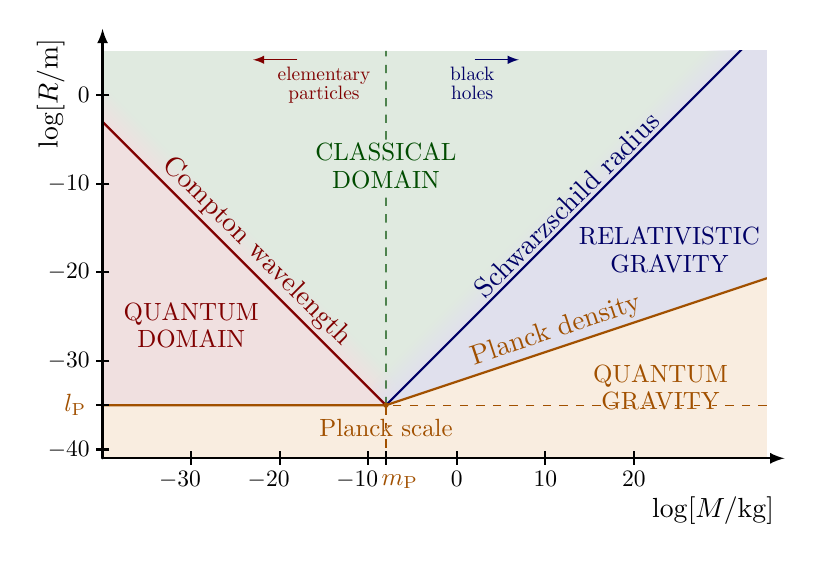
\begin{tikzpicture}[
    scale=0.1,x=32,y=32, % scale such that coordinates coincide with loglog
    every node/.style={align=center}, % for breaking lines in nodes
  ]
  \def\xmin{-40}
  \def\xmax{35}
  \def\ymin{-41}
  \def\ymax{5}
  \def\LP{-35} % Planck length Compton-Schwarschild: sqrt(hbar*G/c^3)
  \def\MP{-8}  % Planck mass Compton-Schwarschild: sqrt(hbar*c/G)
  \def\tick#1#2{\draw[thick] (#1) ++ (#2:25pt) --++ (#2-180:50pt)}
  \coordinate (P) at (\MP,\LP); % Compton-Schwarschild intersection
  \coordinate (C0) at (\xmin,{\LP+(\MP-\xmin)}); % Compton intersection with y axis
  \coordinate (S0) at (\xmax,{\LP+(\xmax-\MP)}); % Schwarschild intersection with y axis
  \coordinate (G0) at (\xmax,{\LP+(\xmax-\MP)/3}); % Quantum gravity intersection with y axis
  
  \begin{scope}
    \clip (\xmin,\ymin) rectangle (\xmax,\ymax);
    
    % REGION FILLS
    \fill[mylightgreen] (\xmin,\ymin) rectangle (\xmax,\ymax);
    %\fill[black!20] (\xmin,\ymin) rectangle (\xmax,\LP+0.01);
    \fill[mylightblue] (P) -- (S0) |- cycle;
    \fill[mylightred] (P) -- (C0) |- cycle;
    \fill[mylightorange] (P) -- (G0) |- (\xmin,\ymin) |- cycle;
    
    % SHADED TRANSITION REGION
    \fill[fill=mylightred,transform canvas={rotate around={45:(P)}},path fading=east]
      (P) rectangle +(3,{2*(\MP-\xmin)});
    \fill[fill=mylightblue,transform canvas={rotate around={-45:(P)}},path fading=west]
      (P) rectangle +(-3,{2*(\xmax-\MP)});
    
    % SCHWARZSCHILD LINE: R = 2GM/c^2 with slope 2G/c^2 = 1.485e-27 m/kg
    \draw[myorange,dashed] (\xmax,\LP) -| (\MP,\ymin); 
    %\draw[myorange] (\MP,\ymin) -- (P);
    \draw[thick,mydarkblue,line cap=round] (P) -- (S0)
      node[pos=0.5,sloped,above=-2,scale=1] {Schwarzschild radius};
    
    % QUANTUM GRAVITY (Planck density): R ~ LP*(M/MP)^1/3
    \draw[thick,myorange,line cap=round] (\xmin,\LP) -- (P) -- (G0)
      node[pos=0.46,sloped,above=-2,scale=1] {Planck density};
    
  \end{scope}
  
  % COMPTON LINE: R ~ hbar/(Mc) with slope hbar/c = 3.519e-43 m.kg
  \draw[dashed,mydarkgreen] (P) -- (\MP,\ymax); % vertical divider
  \draw[thick,mydarkred] (P) -- (C0)
    node[pos=0.5,sloped,above=-2,scale=1] {Compton wavelength};
  \fill[myorange] (P) circle(0.3);
  
  % AXIS
  \draw[->,thick,line cap=round] % log mass (x axis)
    (\xmin,\ymin) -- (\xmax+2,\ymin)
    node[below=10,below left=0] {$\log[M/\si{kg}]$};
  \draw[->,thick,line cap=round] % log radius (y axis)
    (\xmin,\ymin) -- (\xmin,\ymax+2.5)
    node[left=10,above left=0,rotate=90] {$\log[R/\si{m}]$};
  
  % TICKS
  \foreach \x in {-30,-20,...,20}{
    \tick{\x,\ymin}{90} node[left={\x<0?4:0},below=-1,scale=0.85] {$\x$};
  }
  \foreach \y in {-40,-30,-20,...,5}{
    \tick{\xmin,\y}{0} node[left=-1,scale=0.85] {$\y$};
  }
  \tick{\MP,\ymin}{90} node[myorange,right=5,below=0,scale=0.9] {$m_\mathrm{P}$};
  \tick{\xmin,\LP}{0} node[myorange,left,scale=0.9] {$l_\mathrm{P}$};
  
  % REGIMES LABELS
  \node[mydarkgreen,scale=0.9,fill=mylightgreen,inner sep=1] at (\MP,-8)
    {CLASSICAL\\[-1]DOMAIN};
  \node[mydarkred,scale=0.9] at (-30,-26)
    {QUANTUM\\[-1]DOMAIN};
  \node[mydarkblue,scale=0.9] at (24,-17.5)
    {RELATIVISTIC\\[-1]GRAVITY};
  \node[myorange,scale=0.9] at (23,-33)
    %{QUANTUM\\[-1]GRAVITY\\[-1]\contour{mylightorange}{DOMAIN}};
    {QUANTUM\\[-1]\contour{mylightorange}{GRAVITY}}; %\\[-1]DOMAIN};
  \node[myorange,scale=0.9,below=2] at (P)
    {\contour{mylightorange}{Planck scale}};
  
  % LABELS
  \draw[->,mydarkred] (\MP-10,\ymax-1) --++ (-5,0)
    node[pos=0.6,below right,scale=0.7] {elementary\\[-2]particles};
  \draw[->,mydarkblue] (\MP+10,\ymax-1) --++ (5,0)
    node[pos=0.6,below left,scale=0.7] {black\\[-2]holes};
  
\end{tikzpicture}


\end{document}